Generativní modely (\autoref{sec:generative_model}), učení se reprezentací \cite{Bengio2014} a úlohy učení bez učitele (\autoref{sec:unsupervised_learning}) jsou \textbf{klíčové oblastí pro vytvoření inteligentních systémů} \cite{Kingma2019}, \cite{LeCun2022}.
Variační autoenkodér z těchto principů vychází a propojuje je. Ve snaze o konstrukci takového stroje tak variační autoenkodér hraje důležitou roli.

TODO Autoregresivní modely neperspektivní podle LeCun motivace.

\textbf{Variační autoenkodér} \cite{Kingma2014}, \cite{Rezende2014} (dále jen \emph{VAE})
je rámec poskytující metodu pro učení víceúčelových hlubokých modelů využívajících latentních proměnných (\autoref{sec:latent_variable_models})
a příslušných odvozovacích modelů
za použití stochastického gradientního sestupu. \cite{Kingma2019}

VAE nalézá širokou škálu aplikací v generativním modelování, učení se reprezentací a úlohách učení se bez učitele (resp. semi-supervizovaných úlohách).

\section{Motivace vzniku: variační autoenkodér jako generativní model}
Velmi aktuálním tématem v odvětví strojového učení je generativní versus diskriminativní modelování.
V diskriminativním modelování je cílem naučit se prediktor na základě pozorování.
V generativním modelování je cíl poněkud obecnější – naučit se spojité rozdělení pravděpodobnosti skrze všechny proměnné.

Generativní model simuluje způsob, kterým jsou data generována v reálném světě.
\emph{Modelováním} se ve vědních disciplínách rozumí odhalování generujícího procesu stanovením hypotéz a následném testování těchto hypotéz pozorováním
\footnote{For instance, when meteorologists
model the weather they use highly complex partial differential equations
to express the underlying physics of the weather. Or when an astronomer
models the formation of galaxies s/he encodes in his/her equations of
motion the physical laws under which stellar bodies interact. The same
is true for biologists, chemists, economists and so on. Modeling in the
sciences is in fact almost always generative modeling.}. 
S charakterem generativního modelování je spojena řada užitečných výhod.

První z nich je možnost zabudování známých fyzikálních zákonů a omezení do samotného generativního procesu – 
zatímco neznáme (či nepodstatné) \emph{detaily} můžeme zanedbat formou \emph{šumu}. 
Výsledný model je pak často vysoce intuitivní a dobře interpretovatelný.

Dalším důvodem pro snahu o pochopení generativního procesu dat je, že přirozeně zahrnují kauzální vztahy reálného světa.
Pozorování a využití těchto kauzálních vztahů nabízí schopnost generalizovat v dosud nepozorovaných situacích
\footnote{Například, rozumíme-li generativnímu procesu zemětřesení, můžeme tuto znalost využít v Kalifornii i Čile}.

Zatímco generativní modely se zvládnou učit efektivní reprezentace vstupních dat, mají oproti diskriminativním modelům tendenci činit \textbf{silnější předpoklady}, což vede k \textbf{vyššímu asymptotickému biasu} pakliže se model \textbf{plete}. \cite{Banerjee2007}
Pokud nás zajímá pouze naučení se rozlišovat třídy, a náš model se plete (a každý model se \emph{témeř vždy} do určité míry plete), pak diskriminativní modely v takové úloze (za předpokladu dostatečného množství dat) často vedou k menší chybovosti.

I přesto se vyplatí studovat proces generování dat jako způsob, kterým lze trénovací proces diskriminátoru (např. klasifikátoru) zušlechťovat.
Typickým scénářem je úloha, kdy máme k dispozici množinu vzorků se štítky a řádově větší množinu vzorků bez štítků.
V takové úloze semi-supervizovaného učení lze využít generativního modelu dat k zpřesnění klasifikace. \cite{Kingma2014}, \cite{Soenderby2016}

Generativní modelování může být využito i více obecně. Nad generativním modelováním lze uvažovat jako nad jakousi doprovodnou činností.
Například, predikce bezprostřední budoucnosti nám může pomoct při sestavování užitečných abstrakcí o chování světa, které mohou být následně použity pro řadu dalších úloh predikce.
Hledání rozmotaných (\emph{disentangled}), sémanticky významných a statisticky nezávislých kauzálních faktorů variací dat je obecně známo pod pojmem učení se reprezentací bez učitele (\emph{unsupervised representation learning}).
A \textbf{variační autoenkodéry} jsou pro tento účel hojně uplatňovány.

Na tuto úlohu lze alternativně hledět i jako na implicitní formu regularizace. Nutíme-li vzniklé reprezentace být významnými pro proces generování dat, představujeme bias vůči opačnému procesu (který vstupní data mapuje na neužitečné reprezentace).
Doprovodnou činnost predikce bezprostřední budoucnosti tak lze využít k lepšímu porozumění světa v abstraktní úrovni a tím pádem činit přesnější predikce v pozdější fázi.

\section{Princip variačního autoenkodéru}
Variační autoenkodér lze popsat jako dva provázané, byť \textbf{nezávisle parametrizované} modely: \textbf{enkodér} (resp. rozpoznávací) model – \autoref{sec:vae_encoder} a \textbf{dekodér} (resp. generativní) model – \autoref{sec:vae_decoder}.
Tyto dva modely se vzájemně podporují. Enkodér model generativnímu modelu doručuje aproximaci jeho posteriorních náhodných latentních proměnných,
které jsou potřebné pro úpravu jeho parametrů uvnitř iterace \emph{expectation maximalization} učení.
A opačně, generativní model slouží jako opora pro naučení významných reprezentací vstupních dat enkodér modelem.
Tedy, dle Bayesova pravidla, enkodér je \emph{approximate inverse} generativního modelu.

Jednou z výhod VAE oproti běžné variační inferenci (viz \autoref{sec:probabilistic_models_variational_inference}, dále jen \emph{VI}) je, že enkodér model (také nazývaný inferenční model) je nyní stochastickou funkcí vstupních proměnných.
Na rozdíl od VI, kde má každý datový bod vlastní variační rozdělení pravděpodobnosti, což je při větším množství dat neefektivní,
enkodér používá jednu množinu parametrů pro model vztahů mezi vstupními daty a latentními proměnnými. Tento proces nazýváme amortizovanou inferencí.
Takový enkodér model může být libovolně komplexní, ale stále zůstává přiměřeně rychlým, jelikož již z principu může být realizován jedním dopředným průchodem z vstupu skrze latentní proměnné.
Nevýhodou ale je, že při vzorkování vzniká v gradientech potřebných pro učení tzv. vzorkovací šum. Možná největším přínosem VAE je řešení tohoto šumu použitím tzv. \emph{reparametrizačního triku} – jednoduchou procedurou pro přeorganizování výpočtu gradientů, který snižuje variaci gradientu.

Variační autoenkodér je inspirován Helmholtz Machine \cite{Dayan1995}, což byl první model který využíval enkodér modelu.
Nicméně wake-sleep algoritmus, který byl v návrhu využitý, byl silně neefektivní a neoptimalizoval jednoznačné kritérium.
U VAE tedy pravidla pro učení následují jednoznačnou aproximaci cíle.

Variační autoenkodéry jsou spojením pravděpodobnostních grafických modelů a hlubokého učení.
Generativní model je tvořen bayesovskou sítí ve tvaru $p(\mathbf{x}\mid\mathbf{z})p(\mathbf{z})$
\footnote{Případně, má-li generativní model víc stochastických latentní vrstev, má síť následující hiearchii: $p(\mathbf{x}\mid\mathbf{z}_L) p(\mathbf{z}_L\mid\mathbf{z_{L-1}}) \dots p(\mathbf{z}_1\mid\mathbf{z}_0)$.}.
Podobně, enkodér model je tvořen podmíněnou bayesovskou sítí ve tvaru $q(\mathbf{z}\mid\mathbf{x})$
\footnote{Nebo jako hiearchie, např.: $q(\mathbf{z}_0\mid\mathbf{z}_1) \dots q(\mathbf{z}_L \mid X)$.}.
Každá podmíněná vrstva může být tvořena komplexní (hlubokou) umělou neuronovou sítí, například: $\mathbf{z}\mid\mathbf{x} \sim f(\mathbf{x}, \mathbf{\epsilon})$, kde $f$ je mapování umělé neuronové sítě a $\mathbf{\epsilon}$ je \emph{šum} (náhodná proměnná).
Učící algoritmus VAE je variace klasického \emph{expectation maximization algoritmu}. Ten ale skrze reparametrizační trik provádí zpětnou propagaci skrze všechny vrstvy hluboké umělé neuronové sítě (viz \autoref{sec:reparametrization_trick}).

\subsection{Notace}
\begin{itemize}
    \item $X = \{ x^{(i)} \}^N_{i=1}$: Dataset sestavený z $N$ i. i. d. \footnote{Independent and identically distributed, nezávisle a rovnoměrně rozdělené náhodné veličiny.} vzorků nějaké spojité či diskrétní proměnné $x$. 
    Předpokládáme, že tato data byla vygenerována nějakým náhodným procesem, jenž zahrnuje pozorování spojité náhodné proměnné $z$
    \item $z$: Latentní proměnná (latentní reprezentace), kód.
    \item $p_\theta(z)$: Apriorní rozdělení s parametry $\theta$. Jeho hustota pravděpodobnosti je diferenciovatelná s ohledem na $\theta$ a $z$.
    \item $p_\theta(x|z)$: Podmíněné rozdělení s parametry $\theta$. Jeho hustota pravděpodobnosti je diferenciovatelná s ohledem na $\theta$ a $z$.
    \item Proces náhodného generování dat: Zahrnuje pozorování $z$. Skládá se ze dvou kroků: (1) hodnota $z^{(i)}$ je vygenerována z $p_\theta(z)$; (2) hodnota $x^{(i)}$ je generována z $P_\theta(x|z)$.
    \item $q_\phi(z|x)$: \emph{Recognition model} (viz \autoref{sec:vae_encoder}). Probabilistický enkodér. Na základě datového bodu $x$ produkuje rozdělení pravděpodobnosti skrze možné hodnoty kódu $z$, které jej mohly generovat. Aproximace původního \emph{intractable} podmíněného posteriorního rozdělení $p_\theta(z|x)$.
    \item $p_\theta(x|z)$: Probabilistický dekodér (\autoref{sec:vae_decoder}). Na základě kódu $z$ produkuje rozdělení pravděpodobnosti skrze možné hodnoty korespondující s $x$. Jeho využití je generování nových vzorků dat (viz \autoref{sec:vae_generating_new_data}).
    \item $p_\theta(x, z) = p_\theta(z) p_\theta(x|z)$: Generativní model, ze kterého provádíme vzorkování a snažíme se o odhad jeho marginální věrohodnosti.
\end{itemize}

\section{Vymezení problémové oblasti}
Při řešení \autoref{eq:maximum_likelihood} nastávají tři problémy:
\begin{enumerate}
    \item Jakým způsobem definovat latentní proměnné $z$. Tedy určit jakou informaci budou reprezentovat.
    \item \emph{Intractability}, aneb jak vyřešit integrál skrze $z$. \cite[Sekce 2.1.]{Kingma2014}
    \item Velikost datasetu. Provádět dávkovou optimalizaci skrze všechny datové body je příliš drahá operace. Jak dosáhnout parametrických úprav jednotlivých datových bodů \footnote{Případně \emph{minibatch} dávek.} pomocí metod vzorkování.
\end{enumerate}

Na první problém reaguje \autoref{sec:vae_latent_variable}.
Na druhý problém reaguje \autoref{sec:vae_optimization}. A nákladnost dávkových operací řeší \autoref{sec:reparametrization_trick}.
VAE tedy nabízí definitivní všech představených problémů \autoref{eq:maximum_likelihood}. 

\subsection{Volba latentních proměnných dle typu reprezentace informace}
\label{sec:vae_latent_variable}
Jak zvolit latentní proměnné $z$ které správně zachytí latentní informace obsažené v datech?

Před tím, než model vůbec začne generovat nový vzorek dat (například obrázek ručně psané číslice 0-9) musí provést řadu komplexních rozhodnutí.
Volbu samotné číslice, úhel jejího sklonu, tloušťku tahu a celou řadu dalších stylistických vlastností.
Mezi těmito vlastnosti pochopitelně existují korelace, které model musí rovněž zohlednit
\footnote{Např. číslice napsané v rychlosti budou mít typicky vyšší úhel sklonu, ale menší tloušťku tahu.}.
Je tedy zřejmé, že se chceme vyhnout jakémukoliv explicitnímu zahrnutí těchto vlastností do naučeného modelu.
To znamená, že nečiníme explicitní rozhodnutí o tom, jaké dimenze $z$ kódují jakou vlastnost dat
\footnote{Byť určité rozšířené architektury využívají explicitní volby \emph{určitých} dimenzí $z$ – např. \cite{Kulkarni2015}.}.
Stejně tak se chceme vyhnout jakémukoliv explicitnímu popisu závislostí mezi daty (tzv. popisu jejich latentní struktury) mezi dimenzemi $z$. \cite{Doersch2021}

VAE volí unikátní přístup k řešení výše zmíněných omezení. \textbf{VAE předpokládá, že neexistuje žádná triviální interpretace dimenzí $z$, ale raději usuzuje, že $z$ lze vzorkovat z jednoduchého rozdělení pravděpodobnosti $\mathcal{N}(0, I)$}, kde $I$ je jednotková matice. \cite{Doersch2021}

Jak vzorkovat $z$ z rozdělení pravděpodobnosti $\mathcal{N}(0, I)$?

Libovolné rozdělení pravděpodobnosti s $d$ dimenzemi lze generovat množinou o velikosti $d$ proměnných které mají normální rozdělení a jejich následném mapování skrze dostatečně komplexní funkci
\footnote{Pro detailní popis generování rozdělení o $d$ dimenzích odkazuji na \emph{inversion method} popsanou v \cite{Devroye1986}.}.

Řekněme, že chceme sestavit 2D náhodnou proměnou, jejíž hodnoty leží na kruhu.
Tedy $z$ je 2D a má normální rozdělení. Pak funkce $g(z) = \frac{z}{10} + \frac{z}{\| z \|}$ téměř tvoří kruh.
\autoref{fig:latent_variable_ring_structure} ukazuje $z$ a graf funkce $g$.
Deterministická funkce $g$ naučená ze vstupních dat je naprosto stejná \textbf{strategie, kterou VAE požívá pro vytvoření distribuce generující nové vzorky dat}.  \cite{Doersch2021}

\begin{figure}[H]
    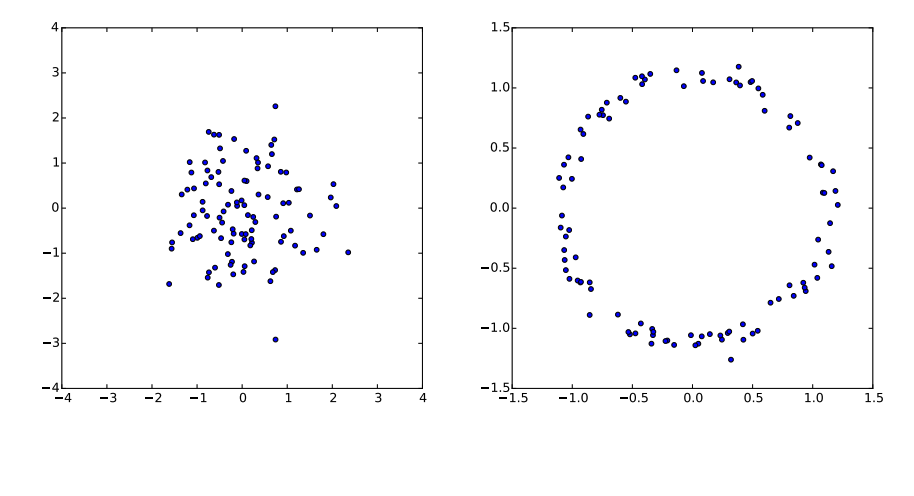
\includegraphics[width=\textwidth]{img/latent_variable_ring_structure.png}
    \caption{Máme-li náhodnou proměnnou $z$ s nějakým rozdělením pravděpodobnosti, můžeme z ní vytvořit zcela novou náhodnou proměnnou $X = g(z)$ s kompletně jiným rozdělením.}
    Levý obrázek zachycuje vzorky z Gaussova rozdělení. Pravý obrázek zachycuje ty stejné vzorky mapované skrze funkci $g(z) = \frac{z}{10} + \frac{z}{\| z \|}$.
    Obrázek včetně interpretace převzaty z \cite{Doersch2021}.
    \label{fig:latent_variable_ring_structure}
\end{figure}

Tedy, má-li VAE k dispozici dostatečně silnou aproximační funkci, může se ze vstupních dat jednoduše naučit funkci, která mapuje nezávislé hodnoty $z$ s normálním rozdělením na libovolné latentní proměnné, které jsou pro model potřebné.
VAE pak takové latentní proměnné mapuje na $X$.   \cite{Doersch2021}

Připomeňme, že (z \autoref{sec:maximum_likelihood}) $P(X|z;\theta) = \mathcal{N}(X|f(z;\theta), \sigma^2 * I)$.
Pokud je $f(z;\theta)$ Vícevrstvý Perceptron (viz \autoref{sec:multilayer_perceptron}), pak si lze intuitivně představit, že jeho umělá neuronová síť využívá svých prvních pár vrstev k mapování normálně rozdělených $z$ na latentní hodnoty (jako např. identita číslice, tloušťka tahu, sklon číslice apod.).
Pozdější vrstvy této sítě mohou být využity k mapování těchto latentních proměnných na obrázek ručně psané číslice (a to sice zcela nově vygenerovaných z pravděpodobnostního rozdělení, viz \autoref{sec:vae_generating_new_data}).
Důležité je, že (obecně) nemusíme řešit zda-li taková latentní struktura ve vstupních datech vůbec existuje.
Pokud nějaká latentní struktura pomáhá modelu s vysokou mírou přesnosti rekonstruovat (tedy optimalizovat ztrátovou funkci, viz \autoref{sec:vae_optimization}) data z trénovací množiny, pak se umělá neuronová síť tuto strukture v \emph{nějaké}\footnote{Za předpokladu dostatečně vysoko-kapacitní umělé neuronové sítě.} vrstvě naučí. \cite{Doersch2021}



